\documentclass{ximera}
\graphicspath{  %% When looking for images,
{./}            %% look here first,
{./pictures/}   %% then look for a pictures folder,
{../pictures/}  %% which may be a directory up.
{../../pictures/}  %% which may be a directory up.
{../../../pictures/}  %% which may be a directory up.
{../../../../pictures/}  %% which may be a directory up.
}

\usepackage{listings}
\usepackage{circuitikz}
\usepackage{xcolor}
\usepackage{amsmath,amsthm}
\usepackage{subcaption}
\usepackage{graphicx}
\usepackage{tikz}
\usepackage{tikz-3dplot}
\usepackage{amsfonts}
\usepackage{mdframed} % For framing content
\usepackage{tikz-cd}

  \renewcommand{\vector}[1]{\left\langle #1\right\rangle}
  \newcommand{\arrowvec}[1]{{\overset{\rightharpoonup}{#1}}}
  \newcommand{\ro}{\texttt{R}}%% row operation
  \newcommand{\dotp}{\bullet}%% dot product
  \renewcommand{\l}{\ell}
  \let\defaultAnswerFormat\answerFormatBoxed
  \usetikzlibrary{calc,bending}
  \tikzset{>=stealth}
  




%make a maroon color
\definecolor{maroon}{RGB}{128,0,0}
%make a dark blue color
\definecolor{darkblue}{RGB}{0,0,139}
%define the color fourier0 to be the maroon color
\definecolor{fourier0}{RGB}{128,0,0}
%define the color fourier1 to be the dark blue color
\definecolor{fourier1}{RGB}{0,0,139}
%define the color fourier 1t to be the light blue color
\definecolor{fourier1t}{RGB}{173,216,230}
%define the color fourier2 to be the dark green color
\definecolor{fourier2}{RGB}{0,100,0}
%define teh color fourier2t to be the light green color
\definecolor{fourier2t}{RGB}{144,238,144}
%define the color fourier3 to be the dark purple color
\definecolor{fourier3}{RGB}{128,0,128}
%define the color fourier3t to be the light purple color
\definecolor{fourier3t}{RGB}{221,160,221}
%define the color fourier0t to be the red color
\definecolor{fourier0t}{RGB}{255,0,0}
%define the color fourier4 to be the orange color
\definecolor{fourier4}{RGB}{255,165,0}
%define the color fourier4t to be the darker orange color
\definecolor{fourier4t}{RGB}{255,215,0}
%define the color fourier5 to be the yellow color
\definecolor{fourier5}{RGB}{255,255,0}
%define the color fourier5t to be the darker yellow color
\definecolor{fourier5t}{RGB}{255,255,100}
%define the color fourier6 to be the green color
\definecolor{fourier6}{RGB}{0,128,0}
%define the color fourier6t to be the darker green color
\definecolor{fourier6t}{RGB}{0,255,0}

%New commands for this doc for errors in copying
\newcommand{\eigenvar}{\lambda}
%\newcommand{\vect}[1]{\mathbf{#1}}
\renewcommand{\th}{^{\text{th}}}
\newcommand{\st}{^{\text{st}}}
\newcommand{\nd}{^{\text{nd}}}
\newcommand{\rd}{^{\text{rd}}}
\newcommand{\paren}[1]{\left(#1\right)}
\newcommand{\abs}[1]{\left|#1\right|}
\newcommand{\R}{\mathbb{R}}
\newcommand{\C}{\mathbb{C}}
\newcommand{\Hilb}{\mathbb{H}}
\newcommand{\qq}[1]{\text{#1}}
\newcommand{\Z}{\mathbb{Z}}
\newcommand{\N}{\mathbb{N}}
\newcommand{\q}[1]{\text{``#1''}}
%\newcommand{\mat}[1]{\begin{bmatrix}#1\end{bmatrix}}
\newcommand{\rref}{\text{reduced row echelon form}}
\newcommand{\ef}{\text{echelon form}}
\newcommand{\ohm}{\Omega}
\newcommand{\volt}{\text{V}}
\newcommand{\amp}{\text{A}}
\newcommand{\Seq}{\textbf{Seq}}
\newcommand{\Poly}{\textbf{P}}
\renewcommand{\quad}{\text{    }}
\newcommand{\roweq}{\simeq}
\newcommand{\rowop}{\simeq}
\newcommand{\rowswap}{\leftrightarrow}
\newcommand{\Mat}{\textbf{M}}
\newcommand{\Func}{\textbf{Func}}
\newcommand{\Hw}{\textbf{Hamming weight}}
\newcommand{\Hd}{\textbf{Hamming distance}}
\newcommand{\rank}{\text{rank}}
\newcommand{\longvect}[1]{\overrightarrow{#1}}
% Define the circled command
\newcommand{\circled}[1]{%
  \tikz[baseline=(char.base)]{
    \node[shape=circle,draw,inner sep=2pt,red,fill=red!20,text=black] (char) {#1};}%
}

% Define custom command \strikeh that just puts red text on the 2nd argument
\newcommand{\strikeh}[2]{\textcolor{red}{#2}}

% Define custom command \strikev that just puts red text on the 2nd argument
\newcommand{\strikev}[2]{\textcolor{red}{#2}}

%more new commands for this doc for errors in copying
\newcommand{\SI}{\text{SI}}
\newcommand{\kg}{\text{kg}}
\newcommand{\m}{\text{m}}
\newcommand{\s}{\text{s}}
\newcommand{\norm}[1]{\left\|#1\right\|}
\newcommand{\col}{\text{col}}
\newcommand{\sspan}{\text{span}}
\newcommand{\proj}{\text{proj}}
\newcommand{\set}[1]{\left\{#1\right\}}
\newcommand{\degC}{^\circ\text{C}}
\newcommand{\centroid}[1]{\overline{#1}}
\newcommand{\dotprod}{\boldsymbol{\cdot}}
%\newcommand{\coord}[1]{\begin{bmatrix}#1\end{bmatrix}}
\newcommand{\iprod}[1]{\langle #1 \rangle}
\newcommand{\adjoint}{^{*}}
\newcommand{\conjugate}[1]{\overline{#1}}
\newcommand{\eigenvarA}{\lambda}
\newcommand{\eigenvarB}{\mu}
\newcommand{\orth}{\perp}
\newcommand{\bigbracket}[1]{\left[#1\right]}
\newcommand{\textiff}{\text{ if and only if }}
\newcommand{\adj}{\text{adj}}
\newcommand{\ijth}{\emph{ij}^\text{th}}
\newcommand{\minor}[2]{M_{#2}}
\newcommand{\cofactor}{\text{C}}
\newcommand{\shift}{\textbf{shift}}
\newcommand{\startmat}[1]{
  \left[\begin{array}{#1}
}
\newcommand{\stopmat}{\end{array}\right]}
%a command to give a name to explorations and hints and theorems
\newcommand{\name}[1]{\begin{centering}\textbf{#1}\end{centering}}
\newcommand{\vect}[1]{\vec{#1}}
\newcommand{\dfn}[1]{\textbf{#1}}
\newcommand{\transpose}{\mathsf{T}}
\newcommand{\mtlb}[2][black]{\texttt{\textcolor{#1}{#2}}}
\newcommand{\RR}{\mathbb{R}} % Real numbers
\newcommand{\id}{\text{id}}


\author{Zack Reed}
%borrowed from Dirk Colbry's msu python stuff
\title{Rank and Nullity}
\begin{document}
\begin{abstract}

In this activity, we will explore the rank and nullity of a matrix.

\end{abstract}
\maketitle

\begin{exploration}

    Let's start with a little warm up exploration! We'll think in $\mathbb{R}^2$ for now.
    
    Remember that linear transformations are completely determined by where they send the standard basis vectors ($\vec{i}$ and $\vec{j}$ for $\mathbb{R}^2$), and that it's possible to determine $\vec{i}$ and $\vec{j}$ such that you can't span all of $\mathbb{R}^2$ from the image of the transformation.

    Go back to the 2D linear transformation GeoGebra applet from before and set $S(\vec{i})$ and $S(\vec{j})$ such that the image of $S$ is a 1-dimensional subspace of $\mathbb{R}^2$ (i.e. a line).
    
    \geogebra{wypahbvn}{800}{600}

    Now, we're going to try to answer a very specific question in this section: What vectors get mapped to $\vec{0}$ by a matrix $A$? Remember that all linear transformations are matrices, so we can reprsent this in the applet by finding vectors $\vec{v}$ such that $S(\vec{v})=\vec{0}$.

    This should be simple enough in the applet, if you set up $S(\vec{i})$ and $S(\vec{j})$ correctly you should be able to hone in on such vectors by rotating $\vec{v}$ around the origin.

    Once you pick up on a few vectors such that $S(\vec{v})=\vec{0}$, try to describe the set of all such vectors. What do you notice about them? Is the set of all such vectors an eclectic collection, or is there a pattern?

    \begin{solution}

        One example is to set $S(\vec{i})=\begin{bmatrix} 1 \\ -1 \end{bmatrix}$ and $S(\vec{j})=\begin{bmatrix} -1 \\ 1 \end{bmatrix}$. The image of $S$ is the line $y=-x$. Vectors $\vec{v}$ whose coordinates are the same, such as $\begin{bmatrix} .38 \\ .38 \end{bmatrix}$ in the figure below, get mapped to $\vec{0}$. Otherwise, vectors get mapped to points on the line $y=-x$. 

        %insert figure
        \begin{center}
            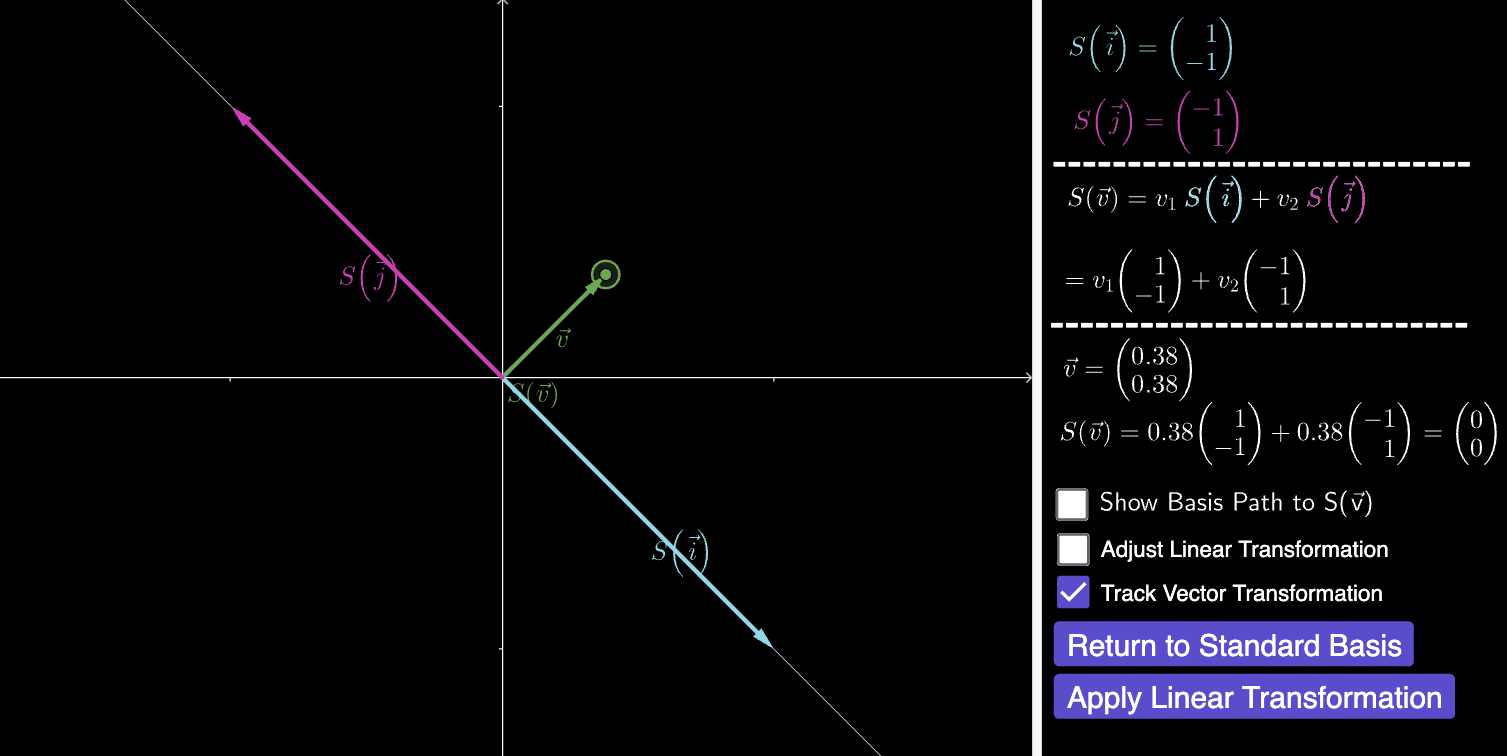
\includegraphics[width=\textwidth]{null_space_1.png}
        \end{center}
    
        In fact, all vectors whose coordinates agree lie along the line $y=x$, so we've found that only vectors within the 1-dimensional subspace spanned by $\begin{bmatrix} 1 \\ 1 \end{bmatrix}$ get mapped to $\vec{0}$. This is an example of what's called a \emph{null space} of a matrix, which we'll explore more in the next few problems.

    \end{solution}

\end{exploration}

Let's start to more systematically explore the idea of a null space in $\mathbb{R}^3$.

Consider the following matrix $A$. 

$$ 
\left[
\begin{matrix}
    1 & 0 & 3  \\
    0 & 1 & 5  \\
    1 & 1 & 8 
\end{matrix}
\right] 
$$

\begin{remark}

    Notice that the third column of $A$ is a linear combination of the first two columns. If we think about $A$ as a linear transformation $S$, that means that $3S(\vec{i})+5S(\vec{j})=S(\vec{k})$. 
    
    In other words, $S(\vec{k})$ is in the span of $S(\vec{i})$ and $S(\vec{j})$. This is a hint that the image of $A$ is not all of $\mathbb{R}^3$.

    Let's view this in our handy GeoGebra applet to confirm where $A$ sends 3D vectors.

    %Insert GeoGebra applet here

\end{remark}


\begin{problem}{{\bf Warm Up:}}
    What is the reduced row echelon form of $A^T$? This will tell you which vectors span the $Im(A)$ (i.e. ``the image of $A$").
    \begin{solution}
        Since reduced row echelon usually operates with rows, we take the transpose of $A$ to instead talk about its columns, which we've come to primarily associate with the $Im(A)$.
        \[
            A^T = 
            \begin{bmatrix}
            1 & 0 & 1 \\
            0 & 1 & 1 \\
            3 & 5 & 8
            \end{bmatrix}
            \]

        As we said, we can combine the first two rows to generate the third row, so the reduced row echelon form of $A^T$ is

        \[
            \begin{bmatrix}
            1 & 0 & 1 \\
            0 & 1 & 1 \\
            0 & 0 & 0
            \end{bmatrix}
        \]

        This confirms that $Im(A)$ is spanned by $\begin{bmatrix} 1 \\ 0 \\ 1 \end{bmatrix}$ and $\begin{bmatrix} 0 \\ 1 \\ 1 \end{bmatrix}$.

        In the next few examples, we'll provide some commands to help you find the reduced row echelon form of more complicated matrices.
    \end{solution}

\end{problem}

Up to this point we've been focusing mainly on the image of matrices and their properties, but we can actually say much about a matrix in terms of the \emph{pre-image} space. The pre-image space is the set of all vectors $\vec{v}$ that get mapped by $A$ into the image $A\vec{v}$. 

One way to describe why the $Im(A)$ is just a plane is to note that some pre-image vectors get mapped to $\vec{0}$. As it turns out, the set of all vectors that get mapped to $\vec{0}$ is a subspace of $\mathbb{R}^3$. We call it the \emph{null space} of $A$.

Let's see if we can describe the null space of $A$.

\begin{definition}

    The {\bf null space} of a matrix $A$ is the set of all vectors $\vec{v}$ such that $A\vec{v} = \vec{0}$. In more compact notation, we write this as 
    $$\text{Null}(A) = \{ \vec{v} \in \mathbb{R}^3 : A\vec{v} = \vec{0} \}.$$

    \begin{hint}

        Remember that in compact math notation, $\in$ reads "in" and $:$ reads |such that". So in words, $$\text{Null}(A) = \{ \vec{v} \text{ in } \mathbb{R}^3 \text{ such that } A\vec{v} = \vec{0} \}.$$

        Remember that $A\vec{v}$ gives you a vector, because the matrix $A$ is a linear transformation that sends vectors to vectors.

    \end{hint}

\end{definition}


\begin{exploration}{Finding the Null Space of $A$}

Let's think back to how $A$ maps vectors as a linear transformation, and rearrange some variables to figure out how we determine which vectors $\vec{v}$ get mapped to $\vec{0}$. 

With our sample matrix $A=\begin{bmatrix} 1 & 0 & 3 \\ 0 & 1 & 5 \\ 1 & 1 & 8 \end{bmatrix}$, we want to find all vectors $\vec{v} = \begin{bmatrix} v_1 \\ v_3 \\ v_3 \end{bmatrix}$ such that $A\vec{v} = \vec{0}$.

This gives the systme of equations

%write the system with v_1, v_2, v_3
\[
\begin{aligned}
    1v_1 + 0v_2 + 3v_3 &= 0 \\
    0v_1 + 1v_2 + 5v_3 &= 0 \\
    1v_1 + 1v_2 + 8v_3 &= 0
\end{aligned}
\]


\end{exploration}

\begin{problem}{Solving the System to Find the $Null(A)$}

Solve the system of equations to find the null space of $A$. Start by finding the reduced row echelon form of $A$. Feel free to use TECH to help you out!

\begin{solution}
    We'll use MATALB to find the reduced row echelon form of $A$. First we enter $A$ and then use the command \begin{verbatim} rref(A) \end{verbatim} to find the reduced row echelon form.

    %Write A as a matrix in MATLAB in a verbatim environment
    \begin{verbatim}
        A = [1 0 3; 0 1 5; 1 1 8]
        reduced=rref(A)
    \end{verbatim}

    This generates the output

    $$A=\begin{bmatrix} 1 & 0 & 3 \\ 0 & 1 & 5 \\ 1 & 1 & 8 \end{bmatrix}$$

    $$\text{reduced}=\begin{bmatrix} 1 & 0 & 3 \\ 0 & 1 & 5 \\ 0 & 0 & 0 \end{bmatrix}$$

\end{solution}

This tells us that $v_3$ is a free variable. When $v_3=1$, we get the system 

\[
\begin{aligned}
    v_1 + 3v_3 &= v_1+3&=0 \\
    v_2 + 5v_3 &= v_2+5&=0
\end{aligned}
\]

which is only solved when $v_1=-3$ and $v_2=-5$. Therefore, the vector $\begin{bmatrix} -3 \\ -5 \\ 1 \end{bmatrix}$ gets mapped to $\vec{0}$.

In fact, any scalar multiple of this vector gets mapped to $\vec{0}$ as well, so if we generally let $v_3=\tau$, then we've determined that any vector of the form $\tau \begin{bmatrix} -3 \\ -5 \\ 1 \end{bmatrix}$ gets mapped to $\vec{0}$. 

We've found the null space! $Null(A)$ is the set of all vectors of the form $\tau \begin{bmatrix} -3 \\ -5 \\ 1 \end{bmatrix}$.

\end{problem}

\begin{remark}

    The collection of the form $\tau \begin{bmatrix} -3 \\ -5 \\ 1 \end{bmatrix}$ is exactly the span of the vector $\begin{bmatrix} -3 \\ -5 \\ 1 \end{bmatrix}$, so we haven't just found the null space of $A$, we've also explicitly described $Null(A)$ as the span of a single vector.

    So, more specifically, we can say that $Null(A)=\text{span}\left\{ \begin{bmatrix} -3 \\ -5 \\ 1 \end{bmatrix} \right\}$. In other words, $\begin{bmatrix} -3 \\ -5 \\ 1 \end{bmatrix}$ is the single basis vector for the null space of $A$, and so $Null(A)$ is a one-dimensional subspace of $\mathbb{R}^3$.

\end{remark}

\begin{problem}{Testing the Null Space}

Let's make sure we're not off base! Pick a few scalars, say $\tau=\pi$ and $\tau=e$, and calculate the product $A\left(\tau\begin{bmatrix} -3 \\ -5 \\ 1 \end{bmatrix}\right)$. What do you get?

\begin{solution}

    We can use MATLAB to calculate the product $A\left(\tau\begin{bmatrix} -3 \\ -5 \\ 1 \end{bmatrix}\right)$ for $\tau=\pi$ and $\tau=e$.

    \begin{hint}{MATLAB Code}
    %\revealbutton{Click to see MATLAB code}
        %Write A as a matrix in MATLAB in a verbatim environment
        \begin{verbatim}
            A = [1 0 3; 0 1 5; 1 1 8]
            v=[-3; -5; 1]
            tau = pi;
            A_pi_v=A*(tau*v)
            
            tau = exp(1);
            A_e_v=A*(tau*v)
        \end{verbatim}
    \end{hint}

    Doing so yields

    $$A\pi\vec{v}=\begin{bmatrix} 0 \\ 0 \\ 0 \end{bmatrix}$$

    $$Ae\vec{v}=\begin{bmatrix} 0 \\ 0 \\ 0 \end{bmatrix}$$

    MATLAB can also handle general scalars, so with the code


    \begin{verbatim}
        syms tau
        A_tau_v=A*(tau*v)
    \end{verbatim}

    we get the output

    $$A\tau\vec{v}=\begin{bmatrix} 0 \\ 0 \\ 0 \end{bmatrix}$$
    

\end{solution}

\end{problem}

As it turns out, this process will let you exactly determine the null space for any given matrix, no matter how nice or complex. Let's try it out with a more complicated matrix, $B$, but we'll shortcut the interlude with systems of equations and instead only work with the reduced row echelon form and the known pivots.

\begin{problem}{Finding the Null Space of $B$}

    %write the matrix B
    Let's consider the matrix $B=\begin{bmatrix}
        1 & 3 & 2 & 0 & 0  \\
        0 & 1 & 5 & 2 & 1  \\
        3 & 5 & -14 & -8 &-4  \\
        0 & 0 & 0 & 1 & 1  \\
        \end{bmatrix}$.

    Find a basis for the null space of $B$.

    \begin{solution}

        Let's start with the reduced row echelon form of $B$.

       %Write B as a matrix in MATLAB in a verbatim environment
       \begin{verbatim}
        B = [1 3 2 0 0; 0 1 5 2 1; 3 5 -14 -8 -4; 0 0 0 1 1]
        [R_new, pivcol_new]=rref(B)
    \end{verbatim}

        This generates the output
        
        \[
            B=\begin{bmatrix}
                1 & 0 & -13 & 0 & 3 \\
                0 & 1 & 5 & 0 & -1 \\
                0 & 0 & 0 & 1 & 1 \\
                0 & 0 & 0 & 0 & 0 \\
            \end{bmatrix}
        \]


    $$\text{pivcol\_new}=\begin{bmatrix} 1 & 2 & 4 \end{bmatrix}$$

    Since the pivot columns determine the solution variables (in this case $v_1, v_2, v_4$), the free variables are $v_3$ and $v_5$. 

    Since $B$ is a $4\times 5$ matrix, it maps 5D vectors to 4D vectors. Hence, the input vectors $\vec{v}$ for any product $B\vec{v}$ must be 5D vectors.

    Since $v_3$ and $v_5$ are free variables, we find the null space spanning vectors by setting each to $1$, the other variable to $0$, and solving for any remaining variables, as we did before.

    For instance, if $v_3=1$ and $v_5=0$, we get the system

    \[
    \begin{aligned}
        v_1 - 13v_3 + 3v_5 &= v_1 - 13 + 0 &= 0 \\
        v_2 + 5v_3 - v_5 &= v_2 + 5 - 0 &= 0 \\
        v_4 + v_5 &= v_4 + 0 &= 0
    \end{aligned}
    \]

    So one basis vector for the nullspace is $\begin{bmatrix} 13 \\ -5 \\ 1 \\ 0 \\ 0 \end{bmatrix}$.

    If we set $v_3=0$ and $v_5=1$, we get the null space basis vector $\begin{bmatrix} -3 \\ 1 \\ 0 \\ -1 \\ 1 \end{bmatrix}$.

    So, $Null(B)=\text{span}\left\{ \begin{bmatrix} 13 \\ -5 \\ 1 \\ 0 \\ 0 \end{bmatrix}, \begin{bmatrix} -3 \\ 1 \\ 0 \\ -1 \\ 1 \end{bmatrix} \right\}$.

    \end{solution}

\end{problem}

\begin{remark}

    You might notice that a quick way to find the null space basis vectors is to set each free variable to $1$ and to negate any other elements in the column. This is a quick way to play out the implications of setting each free variable to $1$ and the others to $0$, as we did in the last problem.

    For example, if the reduced row echelon form of $C=\begin{bmatrix} 1 & 2 & 3 & 5 \\ 2 & 1 & 4 &2 \\ 5 & 4 & 11 & 9 \end{bmatrix}$ is 

    $$\begin{bmatrix} 1 & 0 & 5/3 & -1/3 \\ 0 & 1 & 2/3 & 8/3 \\ 0 & 0 & 0 & 0 \end{bmatrix}$$

    then the null space basis vectors are $\begin{bmatrix} -5/3 \\ -2/3 \\ 1 \\ 0 \end{bmatrix}$ and $\begin{bmatrix} 1/3 \\ -8/3 \\ 0 \\ 1 \end{bmatrix}$.

    There are other ways to also find a basis for the null space, such as using the SVD or other decompositions, but this is the most reliable and direct way to find the null space basis vectors.

\end{remark}

\end{document}